\section{Introduction}

\section{Finite Element Modeling} \label{sec:finiteelementdingus}
A finite element simulation was carried out using the software
\texttt{COMSOL Multiphysics 4.3 (4.3.0.233)} (Comsol Inc., Burlington, MA).
Though the source code of COMSOL is not available for scrutinous review,
the following implementation is generic and may be carried out using other
software (e.g.\ \texttt{OpenFOAM}~\cite{jasak2007openfoam},
\texttt{SU2}~\cite{palacios2013stanford}).  Unless otherwise stated,
implementation specific information is applicable to \comsol.

The simulation is done by solving the steady state incompressible Navier
Stokes equations, neglecting turbulence, using finite element analysis in
two dimensions
\begin{align}
 \rho\left(\mathbf{\dot{u}}\cdot \nabla\right)\mathbf{\dot{u}}
 &=\nabla \cdot \left( -\rho \mathbf{I} + \eta \left(\nabla \mathbf{\dot{u}} +
 \left( \nabla \mathbf{\dot{u}}\right)^\mathrm{T}\right)\right) + \mathbf{F}\\
 \rho \nabla \cdot \mathbf{\dot{u}} &= 0
\end{align}
where $\mathbf{\dot{u}}$ is the flow velocity field, $\rho$ is the fluid
density, $\eta = \eta^\prime + \mi\eta^{\prime\prime}$ is the complex
dynamic viscosity, $\mathbf{I}$ is the identity matrix, and $\mathbf{F}$ is
the body force per unit volume.  The computational domain is set up as
shown in \Figure{fig:compgeometry}.
\begin{figure}[h]
 \centering
 \import{qcm/figures/}{geometry.pdf_tex}
 \caption{Two-dimensional computational domain for the finite element simulation.}
\label{fig:compgeometry}
\end{figure}

It is important to note that, because the simulation is two-dimensional,
what is actually simulated are infinite cylinders rather than spheres.  For
Sauerbrey type viscoelastic films, the difference between two- and three-dimensional simulations is negligible.  However, for asperity contacts such
as spheres, the results however qualitatively correct, did not always
result in exact numerical agreement with
experiment~\cite{Vittorias2010489}.  An extended simulation in three
dimensions at some point is warranted.

The left hand (%
\tikz[baseline=-0.75ex]{
 \draw [dash pattern=on 3pt off 2pt on 1pt off 2pt, thick] (0,0) -- (0.5,0);
}) %
is a sliding wall given a tangential velocity of
\begin{equation}
\mathbf{\dot{u}} =
\begin{pmatrix}
	\dot{u}_x\\
	\dot{u}_y
\end{pmatrix}
=
\begin{pmatrix}
	\dot{u}_\parallel\\
	\dot{u}_\perp
\end{pmatrix}
=
\begin{pmatrix}
	0\\
	\mi\omega u_0	
\end{pmatrix}
\end{equation}
where $\omega=2\pi f$ is the angular frequency of oscillation,
$u_0=\SI{1e-2}{\nano\meter}$ the amplitude, $\dot{u}_x=\dot{u}_\parallel=0$
is the parallel velocity component, and
$\dot{u}_y=\dot{u}{\perp}=\mi\omega u_0$ is the tangential velocity
component.
The top and bottom
boundaries
(%
\tikz[baseline=-0.75ex]{
 \draw [dash pattern=on 3pt off 1pt, thick] (0,0) -- (0.5,0);
} )%
are given a periodic flow condition such that their pressure difference
is zero.  The right hand side (%
\tikz[baseline=-0.75ex]{
 \draw [dash pattern=on 1pt off 1pt, thick] (0,0) -- (0.5,0);
}) %
has a zero-slip condition.  The two materials 1, the particle, and 2, the
medium in domains $D_1$ and $D_2$ are assigned a volume force $\mathbf{F}=\mi \omega \rho
\mathbf{\dot{u}}$,
where $\rho$ is the density of the material, (e.g.\ $\rho_1 =
\SI{1.06}{\gram\per\centi\meter\cubed}$ for polystyrene and $\rho_2 =
\SI{1}{\gram\per\centi\meter\cubed}$ for water).  Finally. an initial pressure point
constraint of $p_0=0$ is assigned to the point in the bottom right of the
domain.

The sphere (or, more appropriately, cylinder, since the simulation is two-dimensional) is domain $D_1$ with diameter $d$ and radius $r$ and is
located a distance $s>-r$, measured from the bottom of the sphere, from the
oscillating boundary.  If $s>0$, the sphere does not make contact with the
boundary.  If $s\leq0$, the sphere is truncated at the boundary resulting
in a finite contact radius $r_\mathrm{c}$; this truncation is identified with
a finite contact radius $r_\mathrm{c}$ in terms of contact mechanics.
It is useful to sample in either domain, so
either $r_\mathrm{c}$ or $s$ is swept, converting between them with
\begin{align}
 r_\mathrm{c}\left(s\right) &= \sqrt{2r-s}\sqrt{s}\\
 s\left(r_\mathrm{c}\right) &= \left(r-\sqrt{r^2-r_\mathrm{c}^2}\right)\sgn\left(r_\mathrm{c}\right).
\end{align}
The number density $N_\mathrm{L}$ was controlled by increasing or
decreasing the height of the domain proportional to the size of the sphere.

The materials in the simulation are assigned a complex dynamic viscosity
$\eta = \eta'-\mi\eta''$.  The complex dynamic viscosity is related to the complex bulk modulus
$G=G'+\mi G''$ by
\begin{align}
 \eta = \frac{G}{\mi \omega}
\end{align}
and the loss tangent, the angle of the complex phasor relative to the real axis is
\begin{equation}
 \tan \delta = \frac{G''}{G'}.
\end{equation}

Specific to the stationary solver in \comsol, in the
\texttt{Study$\rightarrow$Stationary Solver$\rightarrow$Advanced} window,
``Allow complex-valued output from functions with real input'' was checked.
Enabling complex-valued output, coupled with the complex valued input for
the body forces produced shear waves in the simulation.

The mesh settings were calibrated in \comsol~for fluid dynamics with a
maximum mesh size of \SI{1e-9}{\meter} along the oscillating boundary.  All
other meshes were generated automatically.  As for the size of the
computational domain, we find that a height (parallel to the oscillating
boundary) of $h=2d$ and width (tangential to the oscillating boundary)
$w=2d$, minimum of \SI{500}{\nano\meter}, produces consistent results with a
minimum of error and computational resources.


\subsection{Extracting Shifts}
Shifts in frequency, $\df$, and bandwidth (half-width at half maximum),
$\dg$, are computed by evaluating the stress-speed ratio of the oscillating
boundary according to the relationship
\begin{equation}
 \frac{\df+\mi\Delta\Gamma}{f_{\mathrm{F}}}=\frac{\mi}{\pi
									Z_{\mathrm{q}}}Z_\mathrm{L} =\frac{\mi}{\pi
																	Z_{\mathrm{q}}}\left<\frac{\sigma}{\dot{u}_\perp}\right>
\label{eqn:comsolextracttwo}
\end{equation}
where $\sigma$ is the complex stress, $\dot{u}_\perp$ is the complex
tangential velocity component, $Z_\mathrm{L}$ is the load impedance, and $\left<\enspace\right>$
denotes a line average along the boundary.  In \comsol, and in the
coordinates of \Figure{fig:compgeometry}, $\sigma$ is \texttt{Total stress,
y component} (\texttt{v}) and $\dot{u}$ is \texttt{Velocity field, y
component}, (\texttt{spf.T\_stressy}).  As in \Equation{eqn:comsolextract},
note again that the stress speed ratio $\left<\sigma/\dot{u}\right>$
is dimensionally equivalent to specific acoustic impedance, also called
``shock impedance'', sound pressure over tangential velocity; the
stress-speed ratio is the impedance of the film.

\subsection{Verification Examples}
The validity of the numerical simulation was checked against two results
for which the response is well known: the extension of a shear evanescent
wave beyond the oscillating boundary and the complex frequency shifts in
the presence of viscoelastic media.

\subsubsection{Shear Evanescent Wave}
The finite element simulation, when set up as described in
\Section{sec:finiteelementdingus} predicts a shear evanescent wave out from
the tangentially oscillating boundary.  The predictions from the finite
element simulation closely match theory~\cite{steinem2007piezoelectric},
shown in \Figure{fig:suppshearwave}.  The theoretical expression for the
shear evanescent wave is taken as~\cite{steinem2007piezoelectric}
\begin{equation}
 \frac{u(x)}{u_0} = \exp\left(-\sqrt{\frac{\mi \rho \omega}{\eta}} x\right),
\end{equation}
where $x$ is the spatial extension from the tangentially oscillating
boundary in the coordinates of \Figure{fig:compgeometry}.  The $1/\me$
penetration depth $\delta$ is
\begin{equation}
 \delta =
 -\left(\Im\left(\sqrt{\frac{\rho\omega}{\mi\eta}}\right)\right)^{-1}.
\label{eqn:suppshearwavedelta}
\end{equation}
In \Equation{eqn:suppshearwavedelta}, $\Im$ represents a function returning
the imaginary component of a complex variable.

With the material properties of water,
$\rho=\SI{1}{\gram\per\centi\meter\cubed}$ and
$\eta=\SI{1}{\milli\pascal\second}$, \Equation{eqn:suppshearwavedelta}
predicts $\delta\approx\SI{252}{\nano\meter}$, in good agreement with the
simulation data shown in \Figure{fig:suppshearwave}.

\begin{figure}[h]
 \centering
\pgfplotsset{
 minor tick num=3,
 footnotesize,
 every
 axis/.style={
 	thick,
  xmin=0,xmax=1e-6,ymin=-0.1,ymax=1.1,
  width=0.71\textwidth,height=0.45\textwidth,
  xticklabel style={/pgf/number format/fixed,
                     /pgf/number format/precision=1},
 },
 xlabel = $y$ distance,
 ylabel = $|\mathbf{\dot{u}}|$,
 x unit = \si{\micro\meter},
 y unit = a.u.,
 max space between ticks=1000pt,
}
\begin{tikzpicture}[baseline]
\begin{axis}
 \addplot [color=Set14qual1, mark=o, each nth point={5}, only marks ] file {qcm/figures/data/evanescentwave_water_comsol.dat};
 \addlegendentry{simulation}
 \addplot [color=Set14qual2,] file {qcm/figures/data/evanescentwave_water_theory.dat};
 \addlegendentry{theory}
\end{axis}
\end{tikzpicture}
\caption{Finite element prediction of a shear evanescent wave at
\SI{5}{\mega\hertz} in a liquid with
$\rho=\SI{1}{\gram\per\centi\meter\cubed}$ and
$\eta=\SI{1}{\milli\pascal\second}$, compared with theory
(\Equation{eqn:viscoshear}).}
\label{fig:suppshearwave}
\end{figure}

\subsubsection{Semi-Infinite Viscoelastic Medium}
A semi-infinite medium will produce a complex response described
by~\cite{kanazawa1985frequency}~\cite{martin1991characterization}, valid
for crystals with one side in contact with a viscoelastic material,
\begin{align}
 \frac{\df+\mi\dg}{f_\mathrm{F}}&=\frac{\mi}{\pi Z_\mathrm{q}}\sqrt{\rho G}\label{eqn:impeqfirst}\\
                                &= \frac{1}{\pi
																																								Z_\mathrm{q}}\frac{\left(-1+\mi\right)}{\sqrt{2}}\sqrt{\omega \rho \eta}.
\label{eqn:impeq}
\end{align}

In terms of the complex dynamic viscosity and shear modulus,
Equations~\ref{eqn:impeqfirst} and \ref{eqn:impeq} can be expressed as
\begin{align}
\frac{\df+\mi\Delta\Gamma}{f_{\mathrm{F}}}&=\frac{\mi}{\pi Z_{\mathrm{q}}}
\frac{\left(-1+\mi\right)}{\sqrt{2}}\sqrt{\rho\omega\left(\eta'-\mi\eta''\right)}\\
&=\frac{\mi}{\pi Z_{\mathrm{q}}}\sqrt{\rho\left(G'+\mi G''\right)}.
\label{eqn:viscoshear}
\end{align}
The simulation geometry was set as described in \Figure{fig:compgeometry}
but without $D_1$ (no cylinder).  Extracted values of $\df$ and $\dg$ are
presented in \Figure{fig:viscosweep} as a function of the viscosity $\eta$
of medium 2.  In \Figure{fig:viscosweep}(a) $\eta'$ is swept for a
Newtonian fluid, $\eta''=0$.  In \Figure{fig:viscosweep}(b) a non-Newtonian
sample is modeled; $\eta'=\SI{1}{\milli\pascal\second}$ and $\eta''$ is
swept.  The excellent agreement with theory demonstrates that the
simulation is applicable for a wide range of materials.

\begin{figure}[h]
\centering
 \pgfplotsset{
  minor tick num=3,
  footnotesize,
  legend style={font=\footnotesize},
  every axis/.style={
   height=0.48\textwidth,
   width=0.48\textwidth,
   thick,
   %ymin = -0.0003,
   %ymax =  0.0003,
   %xmin = -0.0001,
   %xmax = 0.0038,
  },
  max space between ticks=50pt,
 }
 \begin{tabular}{cc}
 \begin{tikzpicture}[baseline]
  \pgfplotstableread{qcm/figures/data/gksimulation.dat}{\datatablea}
  \pgfplotstableread{qcm/figures/data/gktheory.dat}{\datatableb}
  \begin{axis}[
    xlabel = real viscosity $\eta'$,
    x unit = \si{\pascal\second},
    scaled y ticks=base 10:-3,
    ylabel = {$\df$, $\dg$},
    y unit = \si{hertz},
    ylabel absolute,
    restrict x to domain={-0.01:0.6e-2},
    ylabel style={
      %at={(yticklabel* cs:0.25)},
      %xshift=36pt,
      anchor=center,
     },
   ]
   %\addplot table [ y expr=\thisrowno{1} ] {\datatablea};
   \addplot [color=Set14qual2, mark=,] table [ y expr=\thisrowno{1} ] {\datatableb};
   \addplot [color=Set14qual1, mark=, densely dashed] table [ y expr=\thisrowno{2} ] {\datatableb};

   \addplot [color=Set14qual2, mark=o, only marks] table [ y expr=\thisrowno{1} ] {\datatablea};
   \addplot [color=Set14qual1, mark=o, only marks] table [ y expr=\thisrowno{2} ] {\datatablea};

   \draw [color=gray,dashed,semithick] (axis cs:-0.0001,0) -- (axis cs:6e-2,0);
   \node[anchor=north west] at (yticklabel* cs:1) {(a)};

  \end{axis}
 \end{tikzpicture}
 &
 \begin{tikzpicture}[baseline]
  \pgfplotstableread{qcm/figures/data/gksimulation2.dat}{\datatablea}
  \pgfplotstableread{qcm/figures/data/gktheory2.dat}{\datatableb}
  \begin{axis}[
    xlabel = imaginary viscosity $\eta''$,
    x unit = \si{\pascal\second},
    scaled y ticks=base 10:-3,
    ylabel = ,
    y unit = ,
    ylabel absolute,
    %restrict x to domain={0:0.6e-2},
    legend to name=named,
    legend columns=-1,
%    legend entries={%
%     $\df$ theory,
%     $\dg$ theory,
%     $\df$ simulation,
%     $\dg$ simulation,
%    },
    ylabel style={
      %at={(yticklabel* cs:0.25)},
      %xshift=36pt,
      anchor=center,
     },
   ]
   \addplot [color=Set14qual2, mark=,] table [ y expr=\thisrowno{1} ] {\datatableb};
   \addlegendentry{$\df$ theory~~}
   \addplot [color=Set14qual1, mark=, densely dashed] table [ y expr=\thisrowno{2} ] {\datatableb};
   \addlegendentry{$\dg$ theory~~}

   \addplot [color=Set14qual2, mark=o, only marks] table [ y expr=\thisrowno{1} ] {\datatablea};
   \addlegendentry{$\df$ simulation~~}
   \addplot [color=Set14qual1, mark=o, only marks] table [ y expr=\thisrowno{2} ] {\datatablea};
   \addlegendentry{$\dg$ simulation~~}

   \draw [color=gray,dashed,semithick] (axis cs:-0.001,0) -- (axis cs:6e-2,0);
   \node[anchor=north west] at (yticklabel* cs:1) {(b)};

  \end{axis}
 \end{tikzpicture}
 \\[1.5cm]
 %\multicolumn{2}{c}{ \ref{named} }
\end{tabular}
\caption{Comparison of $\df$ and $\dg$ versus viscosity $\eta$ for both the
 finite element simulation and \Equation{eqn:impeq}.  (a) $\eta''=0$ and
 $\eta'$ is swept (a Newtonian liquid).  (b)
$\eta'=\SI{1}{\milli\pascal\second}$ and $\eta''$ is swept.}
\label{fig:viscosweep}
\end{figure}

It is of note that the Navier-Stokes approach (which solves for
$\dot{\mathbf{u}}$) does not converge in the limit of a perfectly elastic
material, e.g.\ $G=G'$ or $\eta=\eta''$; these systems are typically solved
for $\mathbf{u}$.  It is perhaps possible to couple these two domains, but
we have not attempted to do so.


\section{Analysis and Prediction}
\subsection{Particles}
\begin{figure}[ht]
\centering
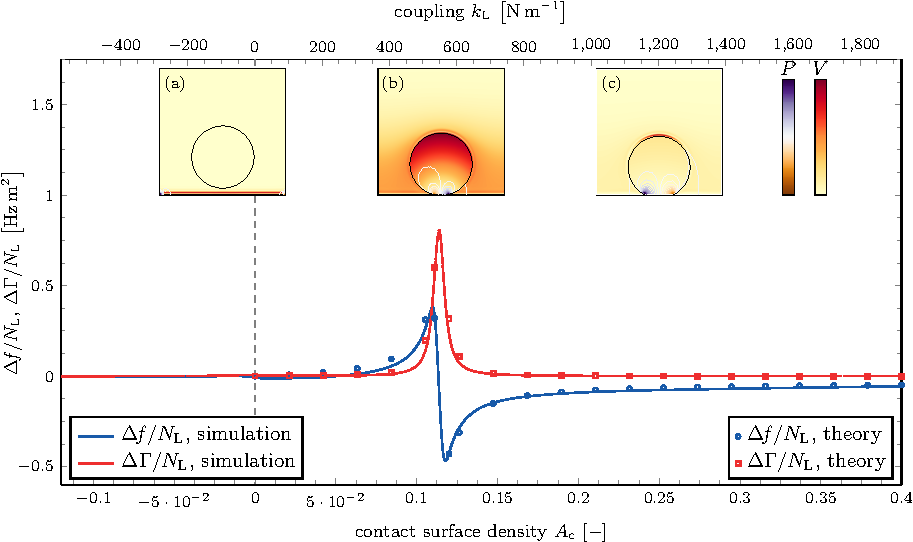
\includegraphics{qcm/figures/lowersphere.pdf}
\caption{%
Simulation of the CF-QCM behavior.
Finite element simulation for a \SI{10}{\micro\meter} polystyrene
sphere (cylinder in 2D) as a function of contact surface density
$A_\mathrm{c}$.  Negative values of $A_\mathrm{c}$ indicate positive
separation from the surface.  Discussion in the text. (a-c): Density plot
of the pressure $P$ and velocity $U$ distributions. Units are normalized.
Note that in all situations with finite contact radius,
stress is annularly distributed around the edge of the contact as per the
Mindlin model~\cite{kumacheva1998interfacial}.
(main plot): Shifts in $\df$ and $\dg$.
Points on the plot are
a best fit of the mechanical model, \Equation{eqn:comsolextract}, to the simulation.}
\label{fig:lowersphere}
\end{figure}

\begin{figure}[ht]
\centering
\import{qcm/figures/}{lowersphere2}
\label{fig:qcmtenvsone}
\end{figure}
A plot of the simulated response in frequency and bandwidth for a
\SI{10}{\micro\meter} particle is depicted in \Figure{fig:lowersphere}.
The spheres were modeled as polystyrene cylinders with density
$\rho=\SI{1.06}{\gram\per\centi\meter\cubed}$, shear modulus
$|G_\mathrm{L}|=\SI{1.3}{\giga\pascal}$, and loss tangent $\tan \delta =
0.001$.  The cylinders are in water with density
\SI{1.0}{\gram\per\centi\meter\cubed} and viscosity
\SI{1.0}{\milli\pascal\second}.  The shifts in $\df$ and $\dg$ are plotted
as a function of a dimensionless contact surface density $A_\mathrm{c}$,
defined as the contact area of the sample per unit area on the oscillating
boundary.

The behavior of the simulation closely matches
experimental observations.  As the cylinder approaches and makes (weak)
contact with the oscillating boundary, a \textit{positive} shift in both
frequency and bandwidth is observed.  As the contact radius increases, the
cylinder becomes more strongly coupled to the boundary. The amount of energy
dissipated into the particle increases until $\dg$ reaches a maximum and
$\df$ experiences a zero crossing.  The limiting case sees a rigid
attachment and the common \textit{negative} frequency shift proportional to
mass adsorption takes hold.
% say here and in the supplement that the velocity component has some phase
% thing

There are two aspects of the simulation that deserve additional
consideration:%
\begin{inparaenum}[(1)]
\item positive shifts in $\df$ and $\dg$ begin
before physical contact with the oscillating boundary and
\item for smaller particles $\dg>\df$ while for
larger particles $\df>\dg$.
\end{inparaenum}

The experiment shows the same behavior, as evidenced in
\Table{tbl:particlesize}.  It is noted however that the procedure of
truncation and its interpretation as finite contact radius in the framework
of contact mechanics utilized on discrete objects are more accurate for
larger particles (\SI{10}{\micro\meter}, as shown in
\Figure{fig:lowersphere}) than smaller ones.  The accuracy discrepancy is
explained in the following way.  It is known in the context of
DVLO\footnote{Derjaguin, Landau, Verwey and Overbeek}
theory~\cite{israelachvili2011intermolecular} that a micron-sized
polystyrene sphere in water near a similarly charged gold surface will
experience a repulsive force due to electrostatic double-layer
effects~\cite{alexander1987hydrodynamic}~\cite{flicker1993quantifying}.
The balance between electrostatic double-layer effects and the
gravitational force determines the height at which the particle will be at
equilibrium above the surface.  For the relevant material
parameters~\cite{israelachvili2011intermolecular}~\cite{sharma1992factors}
it is found that, even at \SI{90}{g}, the smaller \num{1} and
\SI{2}{\micro\meter} particles never make contact with the surface, but
``hover'' at separations of approximately
\SIrange{0.3}{0.15}{\micro\meter}.  At nonzero separations it is posited
that the sphere-surface coupling, being mediated by a viscous liquid, will
be dominated by loss, hence $\dg>\df$.  On the other hand, larger particles
($\sim\SI{10}{\micro\meter}$ and above) with significant mass will overcome
the double-layer forces and make contact with the QCM through a finite
contact radius.  In this case the coupling losses decrease and $\df>\dg$.
%This mechanical model fully describes the behavior of the finite element simulations
%for larger ($d\gtrsim\SI{5}{\micro\meter}$) particles, but fails in the
%limit of smaller particles.

\subsection{Sample Viscoelasticity}
\label{sec:sampleviscoelasticity}
Finally, a comment on the potential of the CF-QCM technique to be
sensitive to different specific viscoelastic properties of discrete samples.  While
the mechanical properties seen in biomaterials spans an enormous
range~\cite{meyers2008biological}, three general categories were chosen to
highlight potentially interesting sensor responses.  As per
\Figure{fig:multisweep} these are: cells~\cite{li2008thickness}, agarose
microparticles~\cite{li2011surface}~\cite{patra2009viscoelastic}, and
protein microcrystals~\cite{zamiri2009modeling}.  Each is treated in the
finite element simulation as a discrete sphere, with complex shear modulus
$G_\mathrm{L}=G_\mathrm{L}'+G_\mathrm{L}''$, where $G_\mathrm{L}'$ is the
storage modulus related to elasticity, and $G_\mathrm{L}''$ is the loss
modulus related to viscosity.  $G_\mathrm{L}$ is related to viscosity
$\eta_\mathrm{L}$ by $\eta_\mathrm{L}=G_\mathrm{L}/(\mi\omegaq)$.  The
shifts in frequency $\df$ and bandwidth $\dg$ are again plotted as a function of
the dimensionless contact surface density $A_\mathrm{c}$.
A fictitious negative $A_\mathrm{c}$
is identified with a finite separation distance from the
simulated QCM surface.  In all cases the coverage ratio was
\SI{50}{\percent}, and furthermore it is assumed that centrifugal force will act to
``push'' the sample into the QCM surface, increasing $A_\mathrm{c}$ and
thus the rigidity of its contact with the QCM.
\begin{figure}[ht]
 \centering
	% height=2.43cm for side pictures, 4cm for axis
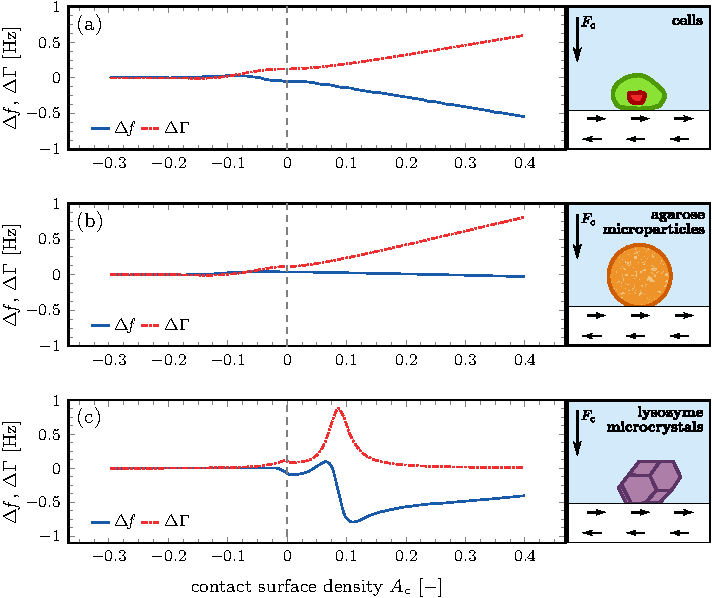
\includegraphics{qcm/figures/multisweep.pdf}
\caption{Simulated response for different materials.  Finite element simulation of normalized $\df$ and $\dg$ for three
 categories of samples as a function of contact surface density,
 $A_\mathrm{c}$.
	Negative values of $A_\mathrm{c}$ indicate the sample has not made contact with the sensor
 surface.
 The samples are (a) cells, $G_\mathrm{L}=\SI{10+50i}{\kilo\pascal}$, (b)
 agarose microparticles, $G_\mathrm{L}=\SI{78+78i}{\kilo\pascal}$ and (c) lysozyme
 microcrystals, $G_\mathrm{L}=\SI{0.659+0.235i}{\giga\pascal}$.  }
\label{fig:multisweep}
\end{figure}

As can be seen, the simulated response of the CF-QCM is markedly different
in each case. Cells, shown in \Figure{fig:multisweep}(a), are assigned a
shear modulus of
$G_\mathrm{L}=\SI{10+50i}{\kilo\pascal}$~\cite{li2008thickness}~\cite{mahaffy2004quantitative} and density
$\rho_\mathrm{L}$ equal to the surrounding liquid medium.  The high loss
modulus and low storage modulus predict the cell will exhibit shifts
characteristic of a viscous fluid.  Likewise, the simulation shows $\df$
and $\dg$ decrease and increase linearly proportional to the contact
parameter, beginning before physical contact occurs.  The proportionality
is a simple function of the shear modulus and density in the
semi-infinite approximation~\cite{flanigan2000contact}~\cite{kanazawa1985frequency}
\begin{equation}
 \frac{\df+\mi\dg}{f_\mathrm{F}}=\frac{\mi}{\pi Z_\mathrm{q}}\sqrt{\rho_\mathrm{L} G_\mathrm{L}}
 \left(A_\mathrm{c}\right)
\end{equation}
 Cells in and of
themselves span a large range of viscoelastic properties which have been
demonstrated to be predictive for diseases such as
cancer~\cite{rebelo2013comparison}.  If one knows the way with which
$A_\mathrm{c}$ is modulated by an applied force (e.g.\ viscoelastic
compliance), linear fitting to
the CF-QCM response will recover $G_\mathrm{L}$ or $\rho_\mathrm{L}$.

Next, \Figure{fig:multisweep}(b) shows the simulated response of agarose
microparticles with a complex shear modulus of
$G_\mathrm{L}=\SI{78+78i}{\kilo\pascal}$~\cite{yao1999situ}~\cite{dimitriadis2002determination}.
Again the density was assumed to be the same as the surrounding medium.
Similar to the viscous behavior of cells, $\dg$ decreases linearly with
$A_\mathrm{c}$.  However, in the simulated agarose microparticles, an
equally large elastic term, $G'_\mathrm{L}$, precludes the equally linear
decrease in $\df$ seen for cells.  Instead, $\df$ increases slightly before
contact and decreases slightly.

At the end of the spectrum, \Figure{fig:multisweep}(c) are lysozyme
microcrystals.  These microcrystals are ``hard'', having been assigned a
complex shear modulus of
$G_\mathrm{L}=\SI{0.659+0.235i}{\giga\pascal}$~\cite{zamiri2009modeling}~\cite{guo2008investigation}.
The simulated response of these is similar to what is experimentally
observed with polystyrene microparticles
($G_\mathrm{L}=\SI{1.3}{\giga\pascal}$).  When the microcrystal enters the
acoustic evanescent wave, there is an initial negative shift as the
effective viscosity-density product increases.  At small contact parameters
there is a positive shift in $\df$ and $\dg$.  Increasing the contact
parameter, $\dg$ sees a maximum and $\df$ a zero crossing.  As the
microcrystal becomes strongly coupled to the QCM, the familiar negative
$\df$ is recovered which, as in \Figure{fig:circlefit}, can be used to
determine the particle size or mass.
